\documentclass[12pt,a4paper]{jsarticle}
\usepackage[utf8]{inputenc}
\usepackage[japanese]{babel}
\usepackage{amsmath}
\usepackage{amsfonts}
\usepackage{amssymb}
\usepackage{graphicx}
\usepackage{url}
\usepackage{listings}
\usepackage{xcolor}
\usepackage{geometry}
\usepackage{fancyhdr}
\usepackage{booktabs}
\usepackage{array}
\usepackage{longtable}
\usepackage{here}

% ページ設定
\geometry{left=25mm,right=25mm,top=30mm,bottom=30mm}

% ヘッダー・フッター設定
\pagestyle{fancy}
\fancyhf{}
\fancyhead[L]{システム統合レポート}
\fancyhead[R]{\thepage}
\renewcommand{\headrulewidth}{0.4pt}

% タイトル情報
\title{プログラミング応用 最終課題レポート\\
\large 新システム提案・計画書}
\author{
グループ名:グループ13 フル単\\
メンバー:井田 礼慈(学籍番号:35714012)\\
\quad\quad\quad 大橋 蒼一朗(学籍番号:35714026)\\
\quad\quad\quad 松岡 遼(学籍番号:35714128)\\
}


\begin{document}

\maketitle

\section{システムの概要}
本提案は、手話を自然な日本語に変換し、音声で読み上げるインタラクティブなコミュニケーション支援システムの開発計画である。主に聴覚障害者と健聴者の間の円滑な会話を実現することを目的とし、手話映像をAIが認識し、適切な日本語文に変換した上で、音声出力を行う。
\section{背景}

% 現在のシステムやプロセスにおける問題点を記述
日本では手話が主要なコミュニケーション手段である一方、手話に対応できる人材が限られているため、聴覚障害者と健聴者との間で意思疎通が困難な場面が多い。特に公共の場や日常生活において、支援者が不在の際に孤立を生む要因にもなっている。これをテクノロジーで補完する必要性が高まっている。


\section{目的}

% プロジェクトの全体的な目標を記述
このシステムの開発目的は、手話利用者が健聴者と対等にコミュニケーションを行える環境を整えることである。手話を理解できない健聴者との会話を可能にし、情報格差を解消することを目指す。

\section{実現上の課題}

\begin{itemize}
    \item 映像から手話単語を正確に抽出するAIの開発
    \item 単語列を自然な文法の日本語文に構成する自然言語処理
    \item 動きの認識と文脈理解を高めるための精度の向上
    \item セキュリティ
\end{itemize}

\section{解決法}

\subsection{映像から単語への変換}
% 技術的課題に対する解決策を詳述
既存の大規模言語モデル(LLM)をベースに転移学習を施し、手話映像から単語を高精度で抽出する。
\subsection{単語列から自然な文章への変換}
% 提案するシステムのアーキテクチャを説明
抽出された単語列を自然な文章に構成するため、LLMの自然言語処理能力を活用する。
\subsection{精度}
% データ統合の具体的手法を説明
独自開発のモーションキャプチャ手袋を導入し、手指の細かな動きを正確に検出する。\\
翻訳エラーのデータベースへの蓄積・分析に基づき定期的な再学習を行い、地域差や個人差への適応も実現する。
\subsection{セキュリティ}
利用者の映像データは匿名化処理を施し、データベースへの安全な蓄積と解析を実施する。

\section{実装工程表}

\subsection{プロジェクト全体スケジュール}
手話認識システムの開発を2026年4月から2027年8月まで(17ヶ月間)で実施する計画である。

\begin{longtable}{|p{2.5cm}|p{2cm}|p{4.5cm}|p{2.5cm}|}
\hline
\textbf{フェーズ} & \textbf{期間} & \textbf{主要作業} & \textbf{成果物} \\
\hline
\endhead

フェーズ1:企画・設計 & 2026年4月-7月 & 要件定義、基本設計、詳細設計 & 要件定義書、基本設計書、詳細設計書 \\
\hline

フェーズ2:AI開発 & 2026年8月-2027年2月 & 手話データ収集、画像認識AI開発、自然言語変換開発、モーションキャプチャ技術開発 & 手話認識AIモデル、自然言語変換モデル、モーションキャプチャシステム \\
\hline

フェーズ3:アプリ開発 & 2026年11月-2027年5月 & UI/UX設計、フロントエンド開発、バックエンド開発、データベース構築 & ユーザーインターフェース、アプリケーション、データベースシステム \\
\hline

フェーズ4:テスト・導入 & 2027年3月-8月 & 単体テスト、統合テスト、ユーザーテスト、システム移行・導入 & テスト報告書、運用システム、運用マニュアル \\
\hline
\end{longtable}
\newpage
\subsection{詳細マイルストーン}
\begin{enumerate}
    \item 要件定義完了:2024年5月
    \item 基本設計完了:2024年7月
    \item プロトタイプ完成:2024年10月
    \item β版リリース:2025年3月
    \item 本格運用開始:2025年8月
\end{enumerate}

\subsection{並行開発スケジュール}
\begin{table}[h]
\centering
\caption{開発チーム別スケジュール}
\begin{tabular}{|l|c|c|c|c|c|c|}
\hline
\textbf{チーム} & \textbf{4-5月} & \textbf{6-7月} & \textbf{8-10月} & \textbf{11-2月} & \textbf{3-5月} & \textbf{6-8月} \\
\hline
企画チーム & \textbf{要件定義} & 設計支援 & - & - & テスト & 導入 \\
\hline
AIチーム & 調査 & 設計 & \textbf{プロト} & \textbf{開発} & 統合 & 運用 \\
\hline
アプリチーム & 調査 & 設計 & 準備 & \textbf{開発} & \textbf{統合} & 運用 \\
\hline
テストチーム & - & 計画 & 準備 & 準備 & \textbf{テスト} & \textbf{導入} \\
\hline
\end{tabular}
\end{table}


\subsection{プロジェクトガントチャート}
% プロジェクト全体のガントチャートを表示
\begin{figure}[H]
\centering
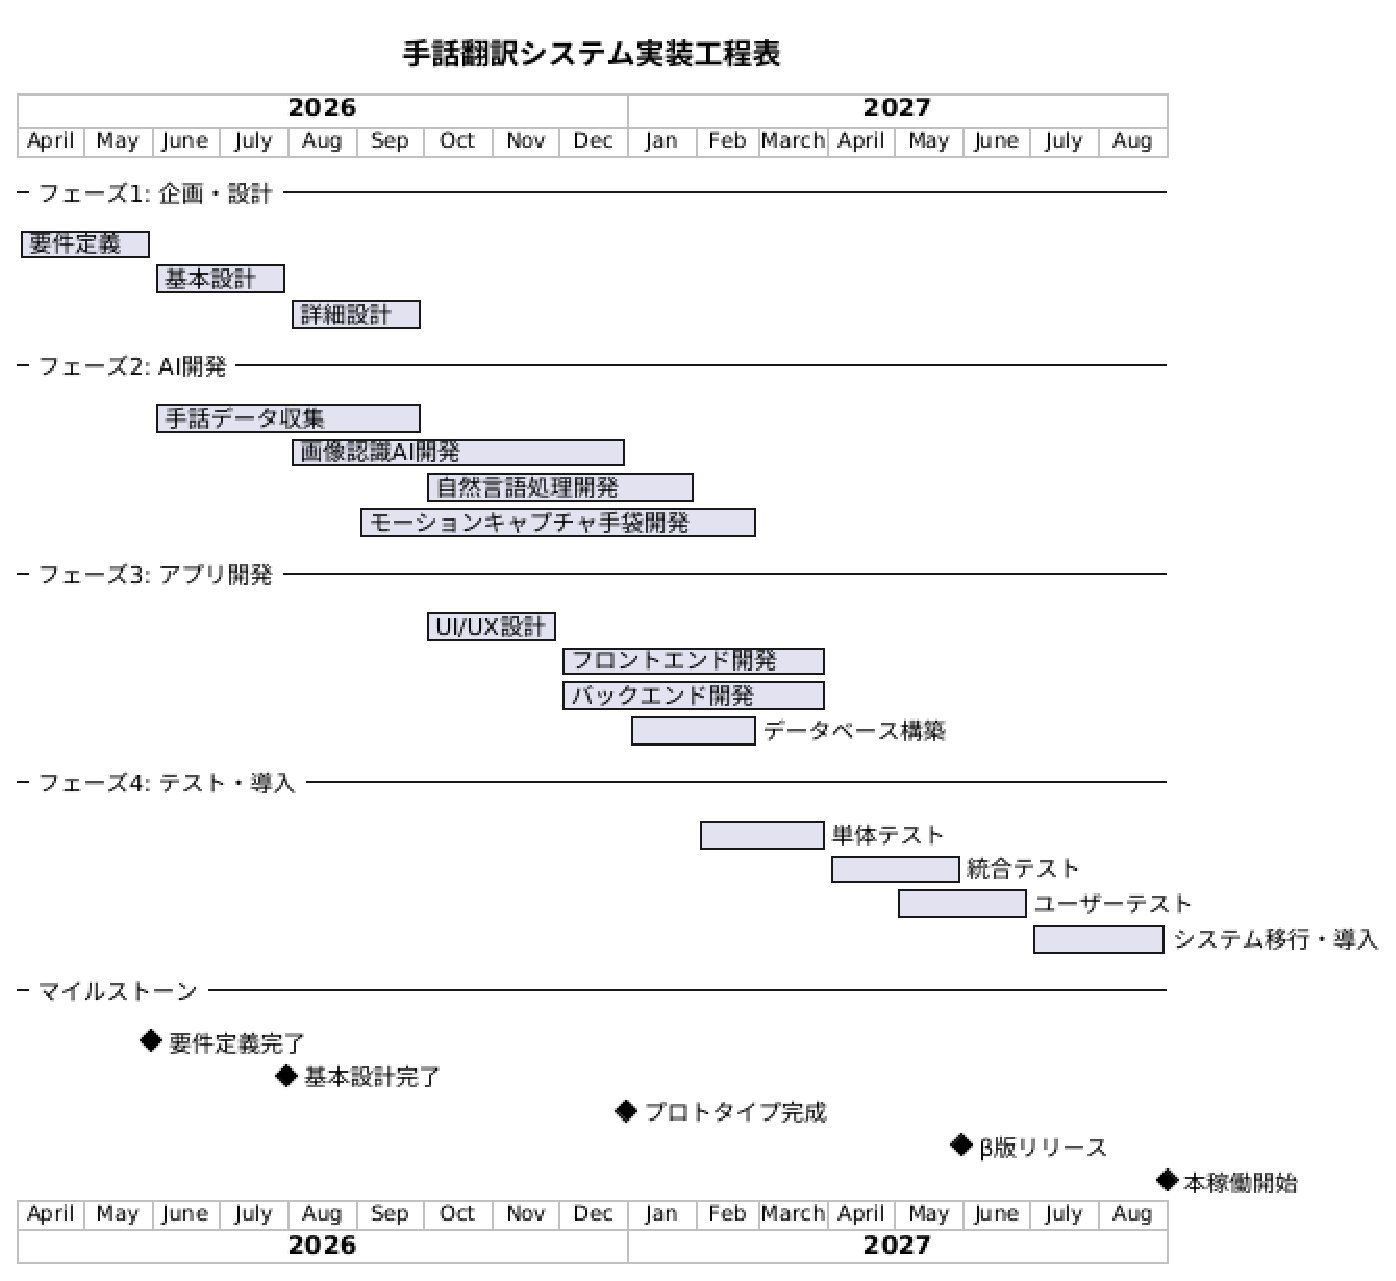
\includegraphics[width=0.85\textwidth]{gantchart.eps}
\caption{手話翻訳システム実装工程表(2026年4月-2027年8月)}
\label{fig:gantchart}
\end{figure}

\section{効果}
このシステムは、手話話者の発言をリアルタイムで自然な日本語に変換・読み上げることで、健聴者との双方向コミュニケーションを実現。特に医療・教育・公共機関などでの活用が期待される。また、地域特有の手話表現への適応力も備えることで、より多様なニーズに応えられる。

\section{まとめ}

手話翻訳システムは、聴覚障害者の社会参加を支援する革新的な技術である。AI技術を核とした本プロジェクトは、誰もが互いに理解し合える社会の実現を目指し、本システムはテクノロジーを通じて対話の可能性を広げる。

\end{document}